\section{VaRTOS, the Variability Aware Real Time Operating System}
\label{sec:vartos}

In this section we outline the implementation of the architecture and algorithms presented in Section \ref{sec:optimization} as a series of extensions to an existing real time operating system (RTOS).  The results shown are using a modified version of the FreeRTOS operating system \cite{freertos}, though the architecture is easily applied to other embedded operating systems as well. The design of VaRTOS must accomplish several key aspects of Section \ref{sec:optimization} while remaining lightweight and energy-efficient.  In particular, VaRTOS includes the following functionality: (1) a method for online modeling of $P_s(T)$ and $P_a(T)$; (2) a method for online modeling of $\mathcal{K}_i$; (3) OS-level control over task knobs $\{k_1,\ldots,k_N\}$; and (4) a tool for evaluating the effects of user inputs $\{k_{i,min},k_{i,max},p_i,E,L\}$ as well as deployment location (temperature profile).  We will describe each of these subsystems in detail below, with various prototypical case studies discussed in Section \ref{sec:casestudies}. 

% Power learning figure
\begin{figure*}
\centering
\subfloat[]{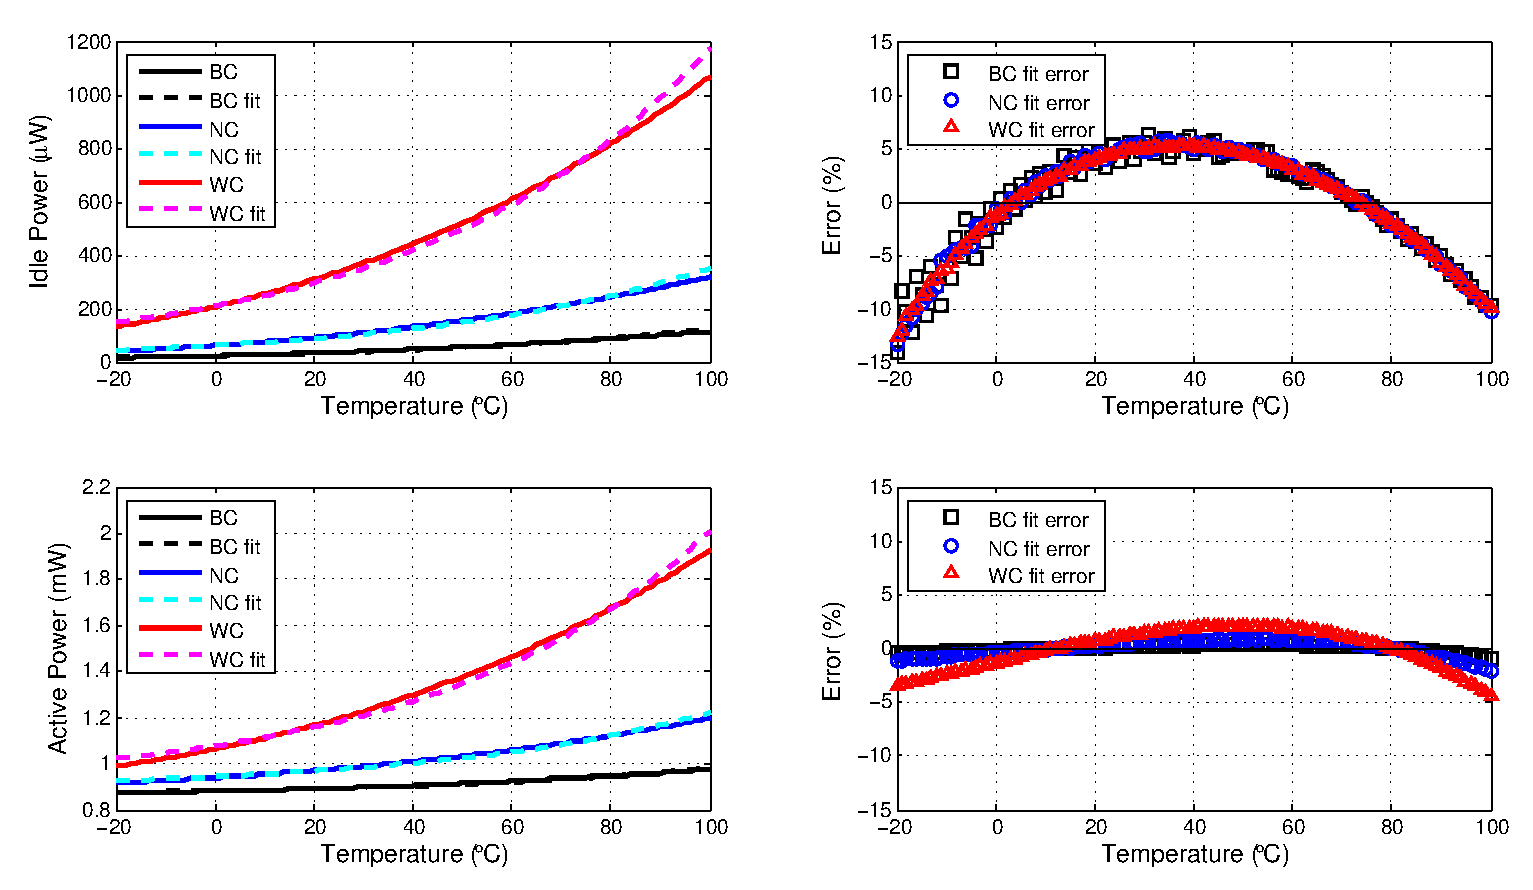
\includegraphics[width=0.47\textwidth, clip=true, trim=0 2.855in 5in 0in]{figures/powerlearning}}
\subfloat[]{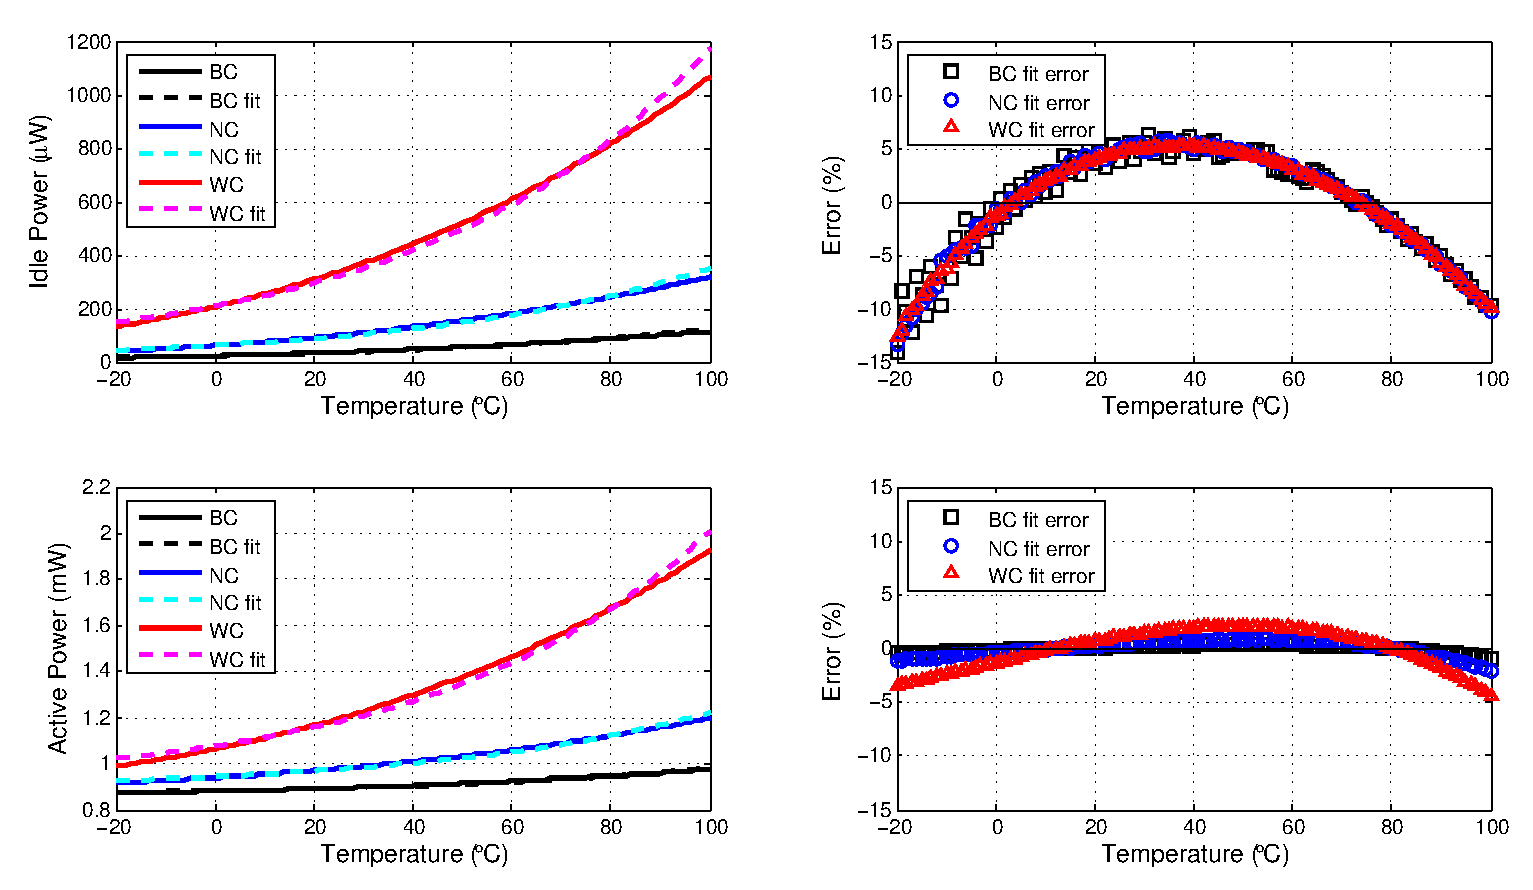
\includegraphics[width=0.47\textwidth, clip=true, trim=5in 2.855in 0in 0in]{figures/powerlearning}}\\
\subfloat[]{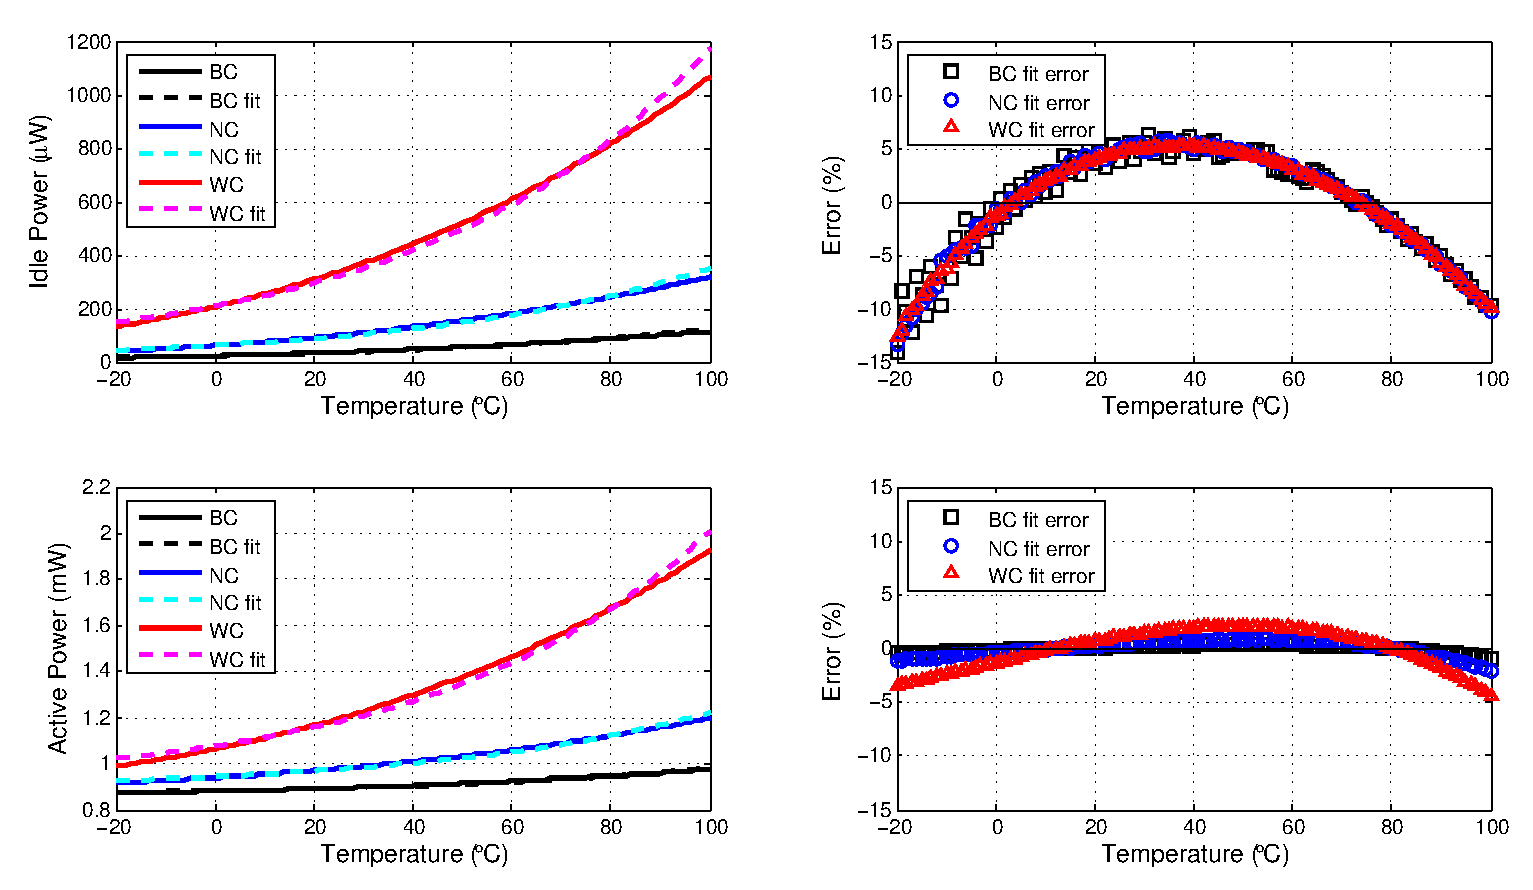
\includegraphics[width=0.47\textwidth, clip=true, trim=0in 0in 5in 2.855in]{figures/powerlearning}}
\subfloat[]{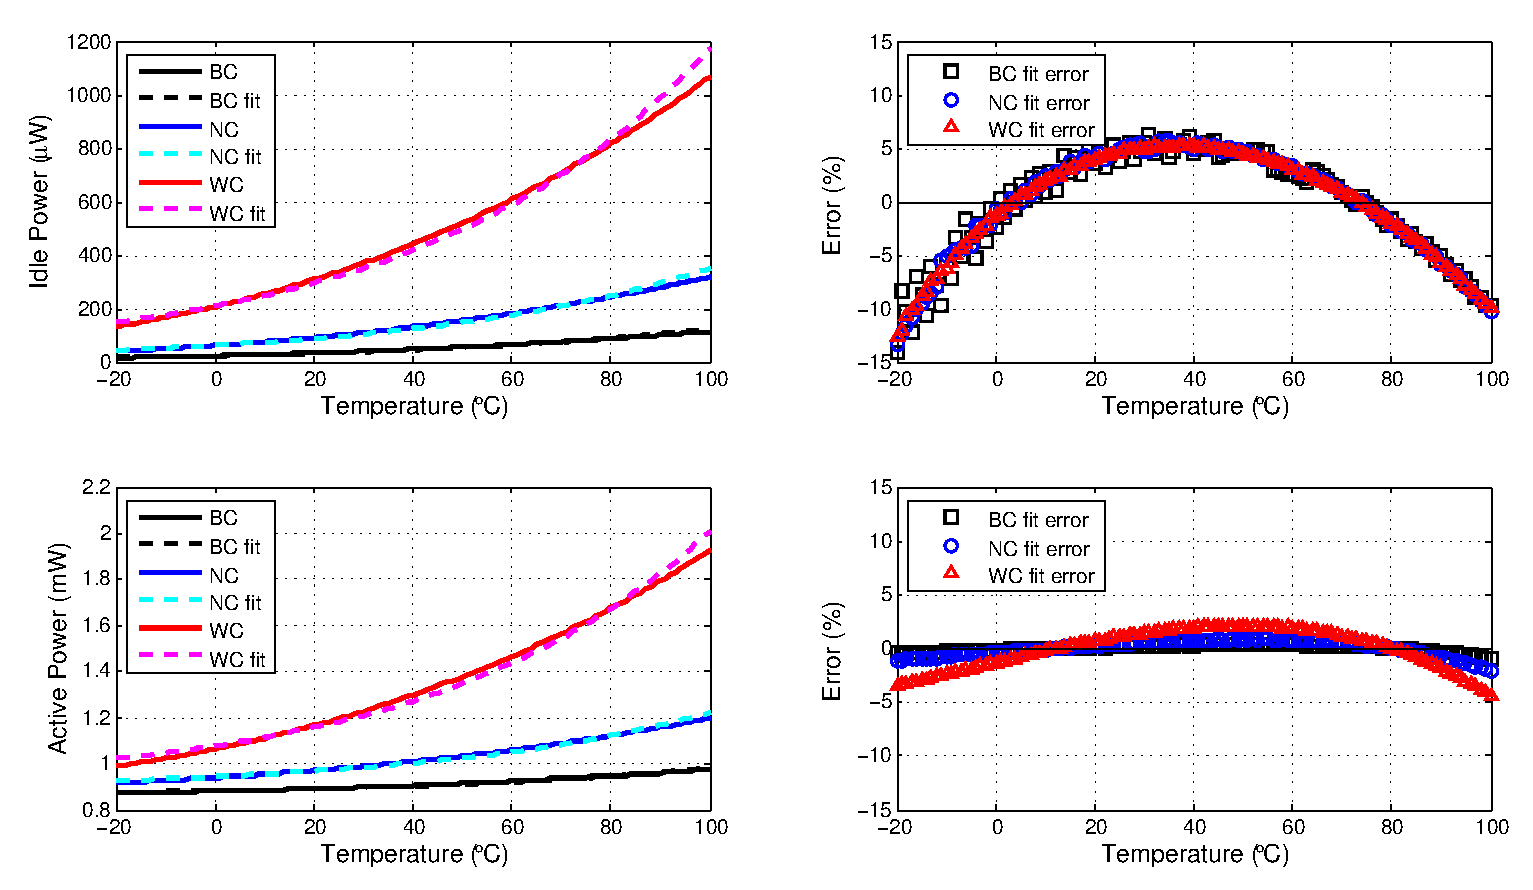
\includegraphics[width=0.47\textwidth, clip=true, trim=5in 0in 0in 2.855in]{figures/powerlearning}}\\ \vspace{0mm}
\caption{\label{fig:powerlearning}Modeling sleep and active power through linearization. }
\end{figure*}

\subsection{Online Modeling of Sleep and Active Power}
As discussed in Section \ref{sec:variability}, both sleep power and active power are nonlinear functions of temperature.  The vast majority of this nonlinearity comes from leakage and sub-threshold currents which dominate in $P_s$. In general, modeling these nonlinear curves could prove difficult with limited resources and without, in many cases, fully fledged math libraries. For example, nonlinear regression is often performed as an optimization problem using a specialized library such as NLopt, requiring more than 300 kB of program space in order to do even rudimentary optimization routines \cite{nlopt} and prohibiting its use in many low power platforms.   Fortunately, the models in Section \ref{sec:variability} describing $P_s$ result in a function that is very closely exponential.  Knowledge of the shape of this function allows us to linearize the model which in turn allows the use of linear regression to accurately model $P_s$.  Specifically, linear regression is run on $\log(P_s)$, giving offset $b_s$ and slope $m_s$.  The desired sleep power model is likewise computed as $P_s(T) \approx \exp(b_s + m_sT)$. After $P_s(T)$ has been computed, $P_a(T)$ can be modeled by subtracting $P_s(T)$ from active power measurements and continuing with a second linear fit.  

The error between the models described in Section \ref{sec:variability} and the linear approximation methods described above is shown in Figure \ref{fig:powerlearning} for three separate power instances representing the best-case (BC), nominal-case (NC), and worst-case (WC) for a 45nm Cortex M3 processor---(a) shows the sleep power model with the corresponding error in (b), and (c) shows the active power model with the corresponding error in (d).  For the linear approximation of $P_s$ on the temperature range [-20$^\circ$C, 100$^\circ$C], the worst case error is around -15\% while on a more temperate range of [0$^\circ$C, 80$^\circ$C] the worst case error is around 5\%.  For most temperature profiles this accuracy will be adequate, but deployments in extreme environments can experience the detriments of errors in the linear model of $P_s$.  Because of the added baseline in $P_a$, the corresponding prediction error is drastically reduced---less than 2\% across [-20$^\circ$C, 100$^\circ$C] for the best-case and nominal instances and less than 5\% for worst-case.  These errors can be further reduced using nonlinear regression methods if the computational resources are not a limiting factor; for VaRTOS we have chosen a lightweight design so that resource-constrained low power processors---those that are likely to be used in long lifetime sensing tasks---can easily perform the necessary computations. 

Models for both $P_s$ and $P_a$ take some time to converge, before which an accurate prediction for the optimal duty cycle $d_{sys}^*$ cannot be calculated. Convergence is aided by variations in temperature, giving a variety of points on the $T\rightarrow\{P_s, P_a\}$ curves, and hurt by noise variance in power sensors.  For example, if our sensor for $P_s$ takes hourly measurements with additive white Gaussian noise $\sim\normal(0, ~5\mu\text{W})$, the percentage error of our model has reached a reasonable accuracy after 40 hours and is nearly fully converged after 60 hours.  This is shown in Figure \ref{fig:powerconvergence} for 190 different locations within the United States with between 1 and 9 years of hourly data in all locations and for processor instances with best-case, nominal-case, and worst-case power consumption. For the results that follow, both sleep and power models will be fit after 40 points (40 hours) of data have been collected.  


\begin{figure*}[t]
\centering
{\centering
\begin{minipage}{0.47\textwidth}
  \centering
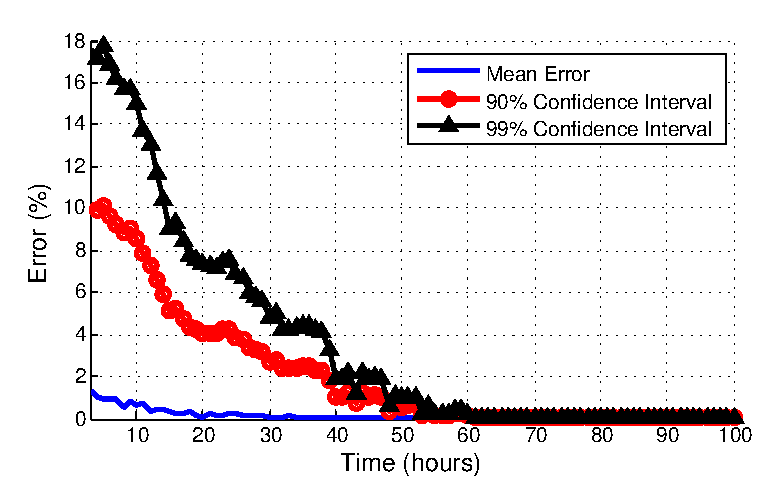
\includegraphics[width=\textwidth]{figures/powerconvergence}
  \captionof{figure}{\label{fig:powerconvergence}Error convergence for sleep power modeling. Shown are the mean errors, 90\% confidence, and 99\% confidence intervals for errors vs. the steady state models. }
\end{minipage}
\hspace{.04\textwidth}
\begin{minipage}{0.47\textwidth}
  \centering
\includegraphics[width=\textwidth]{figures/temperature_estimation_error}
  \captionof{figure}{\label{fig:tempestimation}Error in average power estimation for temperature models constructed from varying numbers of training years ($x$-axis) and with a set number of histogram bins. }
\end{minipage}
}
\end{figure*}

\subsection{Online Modeling of Task Computation}
\label{sec:vartos:knobtime}
Active time per task $t_{a,i}$ can be measured in a number of ways (for example, using hardware timer snapshots at the context swap level).  Given a method for measuring $t_{a,i}$, $\mathcal{K}_i$ is arrived at by systematic perturbation of $k_i$ within the range $[k_{i,min}, k_{i,max}]$. Specifically, $k_i$ is repeatedly increased by $\Delta = {k_{i,max} - k_{i,min} \over n}$ where $n$ is the number of points in the regression, kept sufficiently low ($n = 4$ in our case) to minimize memory footprint.  Between each perturbation in $k_i$, the task is allowed to run for a time period sufficiently long enough to capture active time measurements for tasks with very infrequent activity.  In the applications presented here, this supervisory period is set at $t_{super} = 1$ hour, meaning the mappings $\mathcal{K}_i$ are calculated after 4 hours. Task duty cycles are calculated as $d_i = (\sum t_{a,i})/t_{super}$. Note that $\mathcal{K}_i$ is a linear transformation from $k_i$ to $d_i$ and thus $k_i$ should translate linearly into active time for that task.  In Section \ref{sec:casestudies} we explore the effects of violating this assumption. 

Many tasks are likely to make heavy use of interrupt subroutines (e.g. for analog to digital conversion, radio transmission, serial communication, etc.).  In order for this time to be accounted during the supervisory period, we provide functionality for assigning each subroutine to a particular task using a handle provided during task creation.  For example, on entering a subroutine the \inlinecode{taskEnterISR( taskHandle)} command is invoked with a matching \inlinecode{taskExitISR} upon finishing the subroutine. Again, as mentioned in Section \ref{sec:optimization:maxutil}, in some cases additional peripheral power will be expended during these subroutines.  The metric $t_{a,i}$ reflects only processor power expenditure, and thus peripheral power usage must be modeled separately by modifying $\mathcal{L}_i$. 

\subsection{Controlling Task Active Time}
\label{sec:vartos:tasktime}
In the same way that $k_i$ is perturbed to model $\mathcal{K}_i$ in the previous section, $k_i$ is also commanded by the operating system to achieve $d_i^*$ as calculated by Algorithm \ref{alg}. Knob control is passed from user to operating system at task creation, making the full task creation call using the modified FreeRTOS kernel:

\begin{verbatim}
xTaskCreate( TaskFunction, "name", StackSize, Priority, &TaskHandle,
                                        &TaskKnob, k_min, k_max, p_i);
\end{verbatim}

By its nature, \inlinecode{TaskKnob} serves as a discrete representation of $k_i$ and therefore introduces quantization errors into the optimization routine.  In particular, the smaller the difference between $k_{i,min}$ and $k_{i,max}$, the coarser the granularity of \inlinecode{TaskKnob} becomes and therefore the poorer the achievable resolution of $d_i$ becomes.  As an extreme example, if $k_{i,min} = 1$ and $k_{i,max} = 2$, then \inlinecode{TaskKnob} can only take on 1 of 2 values and thus 1 of 2 $d_i$ values, perhaps far away from $d_i^*$. Similarly, even if \inlinecode{TaskKnob} is constructed in such a way that it has fine granularity, $d_i^*$ might not be within the range $[\mathcal{K}_i[k_{i,min}],~\mathcal{K}_i[k_{i,max}]]$. When $d_i^*$ is less than $\mathcal{K}_i[k_{i,min}]$, task $\tau_i$ consumes more energy than it is allotted and the system is likely to die prematurely.  If $d_i^*$ is greater than $\mathcal{K}_i[k_{i,max}]$, however, it may simply mean that even though additional energy can be allotted to task $\tau_i$, no additional utility would be gained and so achieving a lifetime greater than $L$ is acceptable. 

\subsection{Temperature Models}

Equations \ref{eq:linprog_fin} and \ref{eq:dstar} require that we know the temperature distribution $\pmb{f}_T$ in order to calculate $d_{sys}^*$ and the individual task ratios $\{d_1^*,\ldots,d_N^*\}$. We performed several simulations with results indicating that learning $\pmb{f}_T$ online is infeasible, as it takes the entirety of a year to develop an accurate histogram of the temperature values seen at a given location.  Fortunately, similar simulations show that a very coarse representation of the temperature profile suffices for accurate calculations of $d_{sys}^*$, and furthermore temperature profiles change very little from year to year for a given location. Figure \ref{fig:tempestimation} shows how certain temperature models affect the error in predicting average power consumption for $P_s$ across the lifetime of the system (in this case, 1 year).  The $x$-axis here represents the number of years of temperature data used to train the model before testing on a single year.  Each line represents a certain number of bins used in a histogram representing $\pmb{f}_T$ for a given location. This figure makes two noteworthy points: first, the decreasing estimation error indicates that temperature profiles change very little from year to year, and because of this using multiple years to build $\pmb{f}_T$ only serves to decrease the prediction error in years to come; second, while a 3-bin histogram is inadequate to fully represent the temperature profile for a given location, there is very little benefit in representing $\pmb{f}_T$ with more bins than 5 and even less so with more than 10.  Because of this, for a given location we train with as many previous years as are available and we use a 10-bin histogram to represent $\pmb{f}_T$.  
%Additionally, high resolution is not required on the frequencies of each of these bins, so a single byte per bin suffices, giving a 10 byte representation of the entire temperature profile. This 10 byte histogram is generated \emph{a priori} given a desired deployment location. 


\subsection{User Programming Model}
\label{sec:vartos:tool}
Much of the effort in creating VaRTOS is in making the process transparent to the developer and easing the burden of accounting for variable task power consumption.  In addition to the challenges that come with embedded programming in general, developers need only provide the following information:
(1) Energy budget $E$ measured in Joules;
(2) Lifetime goal $L$ measured in hours;
(3) Deployment location if it belongs in the VaRTOS database or corresponding coarse $\pmb{f}_T$ if not;
(4) $k_{i,min}$, $k_{i,max}$, and priority scaling factors $p_i$;

%Information in (4) above is provided as shown in Section \ref{sec:vartos:tasktime}.  The remaining information is specified as part of a structure that is handed off to the OS scheduling subroutines upon initialization.  
Information required from the developer is therefore very minimal, though in many circumstances it is not readily apparent how different user inputs---particularly for knob values and priorities---will affect the operation of the system.  In order to provide more intuition regarding the various parameters the developer is tasked with supplying, we have developed a simple tool in MATLAB as shown in Figure \ref{fig:gui}.  This tool allows the developer to specify an energy budget and lifetime goal to guide the optimization process.  Developers further specify clock frequency, instance type, a certain geographical location, and the various tasks to be scheduled.  Perhaps the most difficult part of this tool is in estimating how many cycles each task will take per knob value. This tool only gives a rough estimate of how the true deployment will behave, but it helps guide the developer's choices along the way.  

\begin{figure}
\centering
\includegraphics[width=1\textwidth]{figures/matlab_gui}
\caption{\label{fig:gui}A tool for guiding developers using VaRTOS. Users input various system specifications along with task prototypes and a geographical location, and the corresponding optimal duty cycle $d_{sys}^*$ and knobs $k_i^*$ are displayed. }
\end{figure}

\subsection{Operation}
\label{sec:vartos:operation}

\begin{figure}
\centering
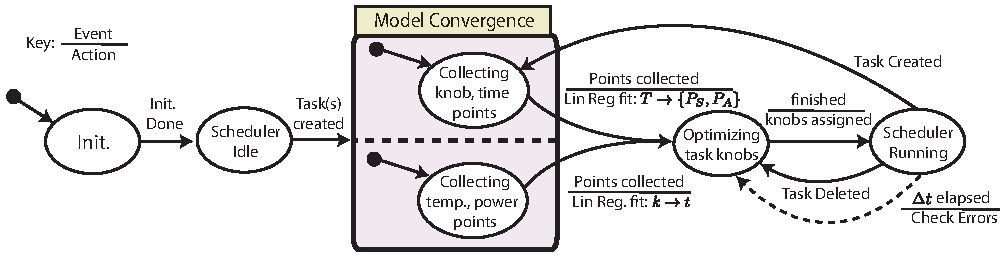
\includegraphics[width=1.0\textwidth]{figures/statechart.pdf}
\caption{\label{fig:statechart}VaRTOS state chart, showing model convergence and optimization states.}
\end{figure}

In this section we discuss the operation of VaRTOS from a broader perspective, using the state chart depicted in Figure \ref{fig:statechart}. To begin, the system is initialized with task creations, energy and lifetime specifications, and a location-specific temperature model.  If at least one task has been created, the scheduler begins operation and we enter a model convergence state.  While in this state, hourly temperature and power measurements are collected and knob values are incremented every $t_{super}$ seconds (see Section \ref{sec:vartos:knobtime}) to construct $\mathcal{K}_i$. The optimization routine cannot complete until both models have converged, after which linear regression and linearization are used to fit the knob to duty cycle and temperature to power curves, respectively. This brings us to the optimization state.  Here the various $d_i^*$ are calculated as per Algorithm \ref{alg}, and the corresponding knob values (calculated by inverting $\mathcal{K}_i$) are assigned to the appropriate tasks. At this point we begin steady state operation in the `Scheduler Running' state. Potential reasons for leaving this state include task creation (necessitating learning the new task's $\mathcal{K}_i$ and re-optimizing) or task deletion (requiring only re-optimization). Because the modeling tasks only run on an as-needed basis, these are implemented as OS tasks with null-valued knobs.  This allows for easy suspension and resumption of these tasks as necessary. 

The dashed line on Figure \ref{fig:statechart} represents an optional feedback error-checking mechanism that can help for online readjustment of poor initial power model construction (e.g. for cases where measurement of $P_s$ and $P_a$ is particularly noisy).  This can be done by comparing true energy expenditure with predicted expenditure, if such a sensor exists, and using the error to apply proportional feedback, though we present no results regarding this extension in this paper. 




%\begin{figure}
%\centering
%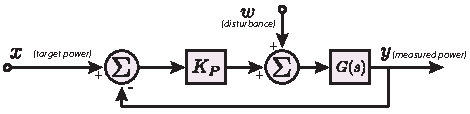
\includegraphics[width=0.5\textwidth]{figures/controlloop.pdf}
%\caption{\label{fig:state chart}state chart}
%\end{figure}




